
%(BEGIN_QUESTION)
% Copyright 2011, Tony R. Kuphaldt, released under the Creative Commons Attribution License (v 1.0)
% This means you may do almost anything with this work of mine, so long as you give me proper credit

En av hovedprosessene i kommunal avløpsrensing er {\it lufting}, der oppløst oksygen i avløpsvannet økes ved å boble luft gjennom vannet i et {\it luftingsbasseng}. En DO-analysator (oppløst oksygen) måler oksygenkonsentrasjonen, og en regulator varierer hastigheten på blåsere som pumper luft inn i bassengene ved hjelp av AC-motorer styrt av frekvensomformere (VFD). VFD-ene gjør at regulatorens 4-20 mA-utgangssignal kan bestemme motorhastigheten:

$$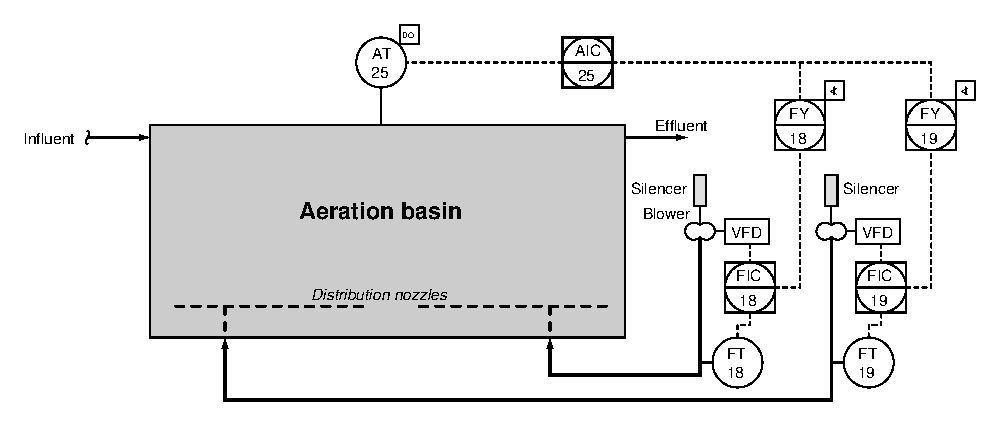
\includegraphics[width=15.5cm]{i00776x01.eps}$$

Angi riktig regulatorvirkning for hver regulator i systemet, forutsatt direktevirkende transmittere og VFD-er som øker motorhastigheten ved større 4-20 mA-signal:

\vskip 10pt

AIC-25 = {\it direkte} eller {\it revers}? \hskip 30pt FIC-18 = {\it direkte} eller {\it revers}? \hskip 30pt FIC-19 = {\it direkte} eller {\it revers}?

\vskip 10pt

Anta at en operatør ber deg undersøke hvorfor DO-verdien ikke holder settpunktet. Ifølge operatøren fungerte alt fint i går, og hadde gjort det i flere måneder. Du går til kontrollrommet og ser disse verdiene i DCS:

% No blank lines allowed between lines of an \halign structure!
% I use comments (%) instead, so that TeX doesn't choke.

$$\vbox{\offinterlineskip
\halign{\strut
\vrule \quad\hfil # \ \hfil &
\vrule \quad\hfil # \ \hfil &
\vrule \quad\hfil # \ \hfil &
\vrule \quad\hfil # \ \hfil \vrule \cr
\noalign{\hrule}
%
% First row
{\bf Parameter} & {\bf AIC-25} & {\bf FIC-18} & {\bf FIC-19} \cr
%
\noalign{\hrule}
%
% Another row
PV & 41\% & 99\% & 2\% \cr
%
\noalign{\hrule}
%
% Another row
SP & 75\% & 100\% & 100\% \cr
%
\noalign{\hrule}
%
% Another row
Output & 100\% & 82\% & 100\% \cr
%
\noalign{\hrule}
} % End of \halign
}$$ % End of \vbox

Identifiser {\it to} ulike feil, der hver av dem alene kan forklare alle symptomene i tabellen.

\begin{itemize}
\item{}
\vskip 50pt
\item{}
\end{itemize}

\underbar{file i00776}
%(END_QUESTION)



%(BEGIN_ANSWER)

{\it To poeng for AIC-virkning, 1 poeng hver for FIC-virkninger. 3 poeng for hver gyldig feil.}

\vskip 10pt

AIC-25 = {\bf revers} \hskip 50pt FIC-18 = {\bf revers} \hskip 50pt FIC-19 = {\bf revers}

\vskip 10pt

Problemet ligger i FIC-19-blåser/dyse-systemet. Muligheter inkluderer:

\begin{itemize}
\item{} Tett dysearrangement
\item{} Tett lyddemper
\item{} VFD-forsyning utløst (av)
\item{} Blåserfeil (blåser ikke luft)
\end{itemize}

%(END_ANSWER)





%(BEGIN_NOTES)

{\bf Dette spørsmålet er ment for eksamen og ikke for arbeidsark!}.

%(END_NOTES)


